In this project, I will present an innovative method useful for computing nonlinear systems. In this case, we are interested in the Lorenz system \cite{Lorenz}, as shown in equation \eqref{eq: lorenz}. Particularly, we will study the stability of the system in order to define a set of chaotic solutions of the Lorenz system. These solutions are represented by the Lorenz Attractor.

This model consists of three ordinary differential equations (ODEs).
\begin{equation}\label{eq: lorenz}
\left\{
\begin{aligned}
\frac{dx}{dt} &= \sigma (y - x) \\
\frac{dy}{dt} &= x (\rho - z) - y \\
\frac{dz}{dt} &= x y - \beta z
\end{aligned}
\right.
\end{equation}
Where $\rho$, $\beta$, and $\sigma$ are three positive parameters. $\sigma$ is known as the Prandtl number, and $\rho$ is called the Rayleigh number. $\beta$ is a geometric parameter.

We will employ a method known as the Multistep Physics-Informed Neural Network \cite{PINNs}. It is based on neural network systems that utilize data from different time steps and physical information to approximate the dynamics of the Lorenz Attractor with a limited amount of noisy data.

\section{Lorenz System}
The Lorenz system is a deterministic and chaotic system. It is highly sensitive to initial conditions, making long-term predictions impossible. The system is also symmetric; if $(x(t), y(t), z(t))$ is a solution, then $(-x(t), -y(t), -z(t))$ is also a solution. The dynamics of the system depend on the choice of parameters, especially on the selection of $\rho$, which determines stability. \\In the subsequent study of fixed points, we will explore how this parameter influences stability.

A \textbf{fixed point} is a point in space such that: 
\begin{equation*}
\left\{
\begin{aligned}
0&= \sigma (y - x) &\Longrightarrow &x=y\\ 
0&= x (\rho - z) - y &\Longrightarrow &(\rho-1-z)x=0\\
0&= x y - \beta z &\Longrightarrow &x^2=\beta z
\end{aligned}
\right.
\end{equation*}
A fixed point can be either stable or unstable. We define a stable point as a point in space from which every perturbation decays exponentially. Conversely, for an unstable point, perturbations grow exponentially. This implies that trajectories will either converge to a point $(x, y, z)$ or diverge as $t$ approaches infinity. The parameter $\rho$ plays a crucial role in determining the stability properties of fixed points.

In this case, we have three fixed points. 
\begin{itemize}
    \item $(0,0,0)$ obtained imposing $z$, $y$ or $x$ equal to zero and it is homogeneous for $\rho<1$. 
    \item imposing $z=\rho - 1 \longrightarrow x^2=\beta(\rho-1)$ for $\rho>1$ we obtain two symmetric points $C^{\pm}=(\pm \sqrt{\beta(\rho-1)},\pm \sqrt{\beta(\rho-1)},\rho-1)$ 
\end{itemize}

To study the nature of a fixed point, we are interested in its eigenvalues. If the real parts of the eigenvalues are negative, the fixed point will be stable; otherwise, it will be unstable.

\section{Stability}
The stability of fixed points in a dynamical system can be analyzed by studying the determinant of the Jacobian matrix.

\begin{equation*}
J(x,y,z) = \begin{bmatrix}
\frac{\partial f_1}{\partial x} & \frac{\partial f_1}{\partial y} & \frac{\partial f_1}{\partial z} \\
\frac{\partial f_2}{\partial x} & \frac{\partial f_2}{\partial y} & \frac{\partial f_2}{\partial z} \\
\frac{\partial f_3}{\partial x} & \frac{\partial f_3}{\partial y} & \frac{\partial f_3}{\partial z}
\end{bmatrix} 
= \begin{bmatrix}
-\sigma & \sigma & 0 \\
\rho - z & -1 & -x \\
y & x & -\beta
\end{bmatrix}
\end{equation*}
where $f_1$, $f_2$ and $f_3$ are the three ODEs of the system.


Now, by computing the Jacobian matrix at the fixed point and evaluating its determinant, we can find the eigenvalues. \\
Starting with the \textbf{point $(0,0,0)$}, we obtain:
\begin{equation*}
J(0,0,0) = \begin{bmatrix}
-\sigma & \sigma & 0 \\
\rho & -1 & 0 \\
0 & 0 & -\beta
\end{bmatrix}
\end{equation*}

\begin{equation*}
Det(J(0)-\lambda 1) = Det\begin{bmatrix}
-\sigma-\lambda & \sigma & 0 \\
\rho & -1-\lambda & 0 \\
0 & 0 & -\beta-\lambda
\end{bmatrix} = 0 
\end{equation*}

\begin{equation*}
    \begin{array}{cc}
        (\beta+\lambda) [(\sigma +\lambda)(1+\lambda)-\sigma \rho]=0\\ 
        (\beta+\lambda) [\lambda^2+\lambda(\sigma+1)+\sigma(1-\rho)]=0
    \end{array}
\end{equation*}
So we have find out three eignevalues:
\begin{itemize}
    \item $\lambda_0=-\beta$. Stability requires $\beta >0 $, which is typically the case in the Lorenz system.
    \item $\lambda_{\pm} = \frac{1}{2}[-(\sigma+1)\pm \sqrt{(\sigma-1)^2 +4 \sigma \rho)}]$. We have to study in which conditions the real parts of $\lambda_{\pm}$ are negative. % if: \\$(\sigma-1)^2 +4 \sigma \rho<0$ this inequality implies $\rho <1+\frac{(\sigma-1)^2}{4\sigma}$ 
    In order to do that we define a new matrix
    \begin{equation*}
        A = \begin{bmatrix}
        -\sigma & \sigma  \\
        \rho & -1 \\
        \end{bmatrix} 
    \end{equation*}
    Let's compute the Trace $Tr(A)=-\sigma -1$ and the Determinant of A, $Det(A)=\simga(1-\rho)$. The real part is negative if and only if $$Tr(A)^2<4Det(A)$$
    In Fig. \ref{fig: Poincaré maps}, we can observe the Poincaré map, which provides us with information on the stability criteria: 
\begin{itemize}
    \item For $\rho<1$, we have $Det(A)=\sigma(1-\rho)>0$, implying a stable node in the plane. There are three real negative eigenvalues, and zero acts as a local attractor.
    \item For $\rho>1$, $Det(A)=\sigma(1-\rho)<0$, indicating a saddle in the plane. We observe two real negative eigenvalues and one real positive eigenvalue. Zero becomes an unstable point.
\end{itemize}
For $\rho<1$ every trajectory approaches the origin as $t \longrightarrow \infty$. It is called globally stable.

\end{itemize}








%the determinant is equal to zero if $\lambda_0=-\beta$ or $\lambda_{\pm} = \frac{1}{2}[-(\sigma+1)\pm \sqrt{(\sigma-1)^2 +4 \sigma \rho)}].$ %$\lambda^2+(\sigma+1)\lambda+\sigma(1-\rho)=0 \longrightarrow \lambda_{\pm} = -\frac{1}{2}[(\sigma+1)\pm \sqrt{(\sigma+1)^2 -4 \sigma(1-\rho)}]$ \\ \longrightarrow \sigma(1-\rho) < \frac{(\sigma+1)^2}{4}
%Knowing that there exist three real eigenvalue we want to classify the type of stability. 
%We define a new matrix
%\begin{equation*}
%A = \begin{bmatrix}
%-\sigma & \sigma  \\
%\rho & -1 \\
%\end{bmatrix} 
%\end{equation*}
%We compute the trace of $A$ and the determinant of $A$ as $Tr(A)=-\sigma-1, \ Det(A)=\sigma(1-\rho)$. Knowing that $Tr(A)^2-4Det(A)>0$ it implies $(\sigma+1)^2-4\sigma(1-\rho)>0$

%------------------------------------------------------

\begin{figure}
\centering    
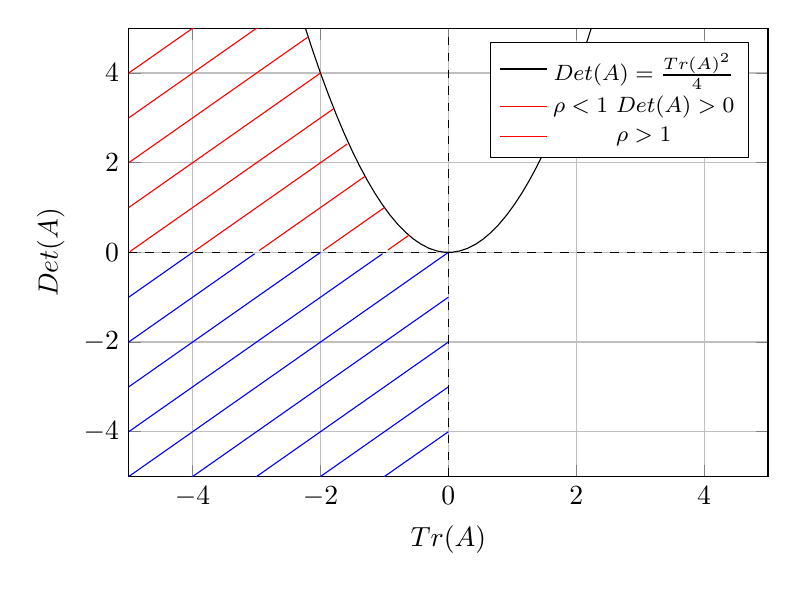
\begin{tikzpicture}
\begin{axis}[
    xlabel={$Tr(A)$},
    ylabel={$Det(A)$},
    grid=major,
    width=0.8\textwidth,
    height=0.6\textwidth,
    xmin=-5, xmax=5,
    ymin=-5, ymax=5,
    legend pos=north east,
    legend style={font=\footnotesize},
    samples=100 % Numero di campioni per disegnare la funzione
]

% Inserisci la tua funzione qui
\addplot[black, domain=-6:6] {x^2};
\addlegendentry{$Det(A)=\frac{Tr(A)^2}{4}$}

\addplot[red,domain=-6:-0.62, restrict y to domain=0:10]{x+1};
\addplot[red,domain=-6:-1, restrict y to domain=0:10]{x+2};
\addplot[red,domain=-6:-1.3, restrict y to domain=0:10]{x+3};
\addplot[red,domain=-6:-1.58, restrict y to domain=0:10]{x+4};
\addplot[red,domain=-6:-1.80, restrict y to domain=0:10]{x+5};
\addplot[red,domain=-6:-2, restrict y to domain=0:10]{x+6};
\addplot[red,domain=-6:-2.2, restrict y to domain=0:10]{x+7};
\addplot[red,domain=-6:-2.58, restrict y to domain=0:10]{x+8};
\addplot[red,domain=-6:-2.58, restrict y to domain=0:10]{x+9};
\addlegendentry{$\rho<1 \ Det(A)>0$}

\addplot[blue,domain=-6:0, restrict y to domain=-10:0]{x-4};
\addplot[blue,domain=-6:0, restrict y to domain=-10:0]{x-3};
\addplot[blue,domain=-6:0, restrict y to domain=-10:0]{x-2};
\addplot[blue,domain=-6:0, restrict y to domain=-10:0]{x-1};
\addplot[blue,domain=-6:0, restrict y to domain=-10:0]{x};
\addplot[blue,domain=-6:0, restrict y to domain=-10:0]{x+1};
\addplot[blue,domain=-6:0, restrict y to domain=-10:0]{x+2};
\addplot[blue,domain=-6:0, restrict y to domain=-10:0]{x+3};
\addplot[blue,domain=-6:0, restrict y to domain=-10:0]{x+4};
\addlegendentry{$\rho>1$}

% Disegna l'asse y=0 e l'asse x=0
\draw[black, dashed] (axis cs:0,\pgfkeysvalueof{/pgfplots/ymin}) -- (axis cs:0,\pgfkeysvalueof{/pgfplots/ymax});
\draw[black, dashed] (axis cs:\pgfkeysvalueof{/pgfplots/xmin},0) -- (axis cs:\pgfkeysvalueof{/pgfplots/xmax},0);

\end{axis}
\end{tikzpicture}
\caption{Stability diagram classifying Poincaré maps}
\label{fig: Poincaré maps}
\end{figure}

%------------------------------------------------------









\vspace{12pt}
%Now suppose $\rho>1$, 
Let's study what happens on the \textbf{points $C^+$ and $C^-$}.
To analyze the stability of these points, we linearize the Lorenz equations around each equilibrium point and compute the Jacobian matrix for the points $C^{\pm}$

\begin{equation*}
J(C^+) = \begin{bmatrix}
-\sigma & \sigma & 0 \\
1 & -1 & - \sqrt{\beta(\rho-1)} \\
\sqrt{\beta(\rho-1)} & \sqrt{\beta(\rho-1)} & -\beta
\end{bmatrix}
\end{equation*}
As we did before, we can determine the eigenvalues computing the following determinant
\begin{equation*}
Det(J(C^+)-\lambda 1) = \begin{bmatrix}
-\sigma -\lambda & \sigma & 0 \\
1 & -1 - \lambda & - \sqrt{\beta(\rho-1)} \\
\sqrt{\beta(\rho-1)} & \sqrt{\beta(\rho-1)} & -\beta - \lambda
\end{bmatrix} = 0 
\end{equation*}

\begin{equation}\label{eq:detC}
    \begin{array}{cc}
         &\lambda^3+(\sigma + \beta +1)\lambda^2+\beta(\rho+\sigma)\lambda + 2\beta\sigma(\rho -1)=f(\lambda)=0
         
    \end{array}
\end{equation}
We can analyze the sign of the eigenvalues graphically. By utilizing software such as Geogebra, we can plot the functions \eqref{eq:detC} and determine the sign by locating their intersections with the y-axis, which varies with $\rho$. In Fig \ref{fig: red and blue lines} we can see a graph like that. The red line describes the case with $\rho=1$ and the blue one with $\rho>1$. In the red case, the intersections with the x-axis tell us that we have 2 distinct negative real eigenvalues and one equal to zero. Otherwise, for $\rho>1$ we find 3 distinct real eigenvalues.




%Let us see what happens if $\rho \longrightarrow 1^+$.
%If $\rho=1 \longrightarrow \lambda[\lambda^2 + (\sigma +\beta+1)\lambda+\beta(1+\sigma)]$. We have three roots
%\begin{itemize}
%    \item $\lambda=0$
%    \item $\lambda_+=-\beta, \lambda_-=-\sigma-1$ %\lambda_{\pm}=\frac{1}{2}[-(\sigma+\beta+1)\pm \sqrt{(\sigma+\beta+1)^2-4\beta(1+\sigma)}]\\=\frac{1}{2}[-(\sigma+\beta+1)\pm \sqrt{(1+\sigma-\beta)^2)}], \
%\end{itemize}
%In Fig. \ref{fig: red and blue lines} we can see a red line for $\rho=1$ and a blue line for $\rho>1$. In the first case, the three intersections with the x-axis tell us that we have 2 distinct real negative eigenvalues and one equal to zero. Otherwise, for $\rho>1$ we find 3 distinct real negative eigenvalues. 
%$\lambda \leq \frac{-2\sigma}{1+\sigma}(\rho-1)$

%------------------------------------------------------
\begin{figure}
\centering    
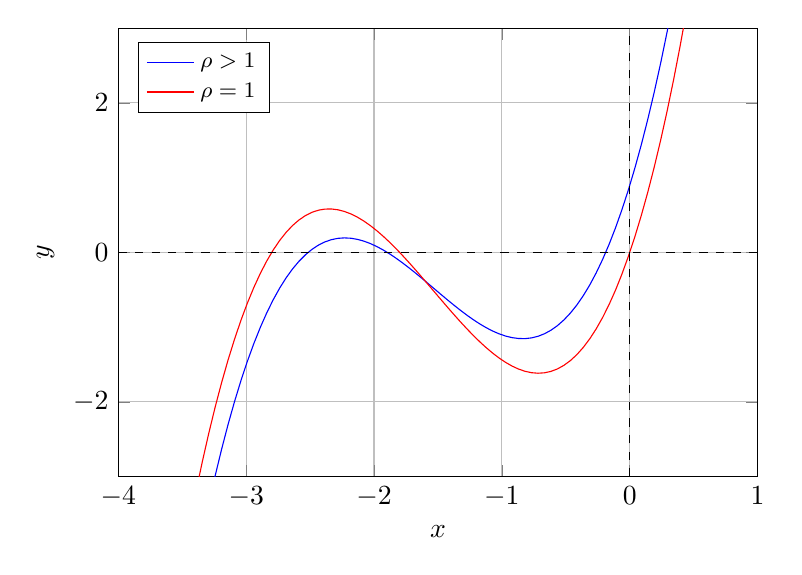
\begin{tikzpicture}
\begin{axis}[
    xlabel=$x$,
    ylabel=$y$,
    grid=major,
    width=0.8\textwidth,
    height=0.6\textwidth,
    xmin=-4, xmax=1,
    ymin=-3, ymax=3,
    legend pos=north west,
    legend style={font=\footnotesize},
    samples=100 % Numero di campioni per disegnare la funzione
]

% Inserisci la tua funzione qui
\addplot[blue, domain=-4:1] {x^3+(0.8+2.8+1)*x^2+2.8*(1.2+0.8)*x+2*0.8*2.8*(1.2-1)}; % Esempio: Grafico della funzione y = x^2
\addplot[red, domain=-4:1] {x^3+(0.8+2.8+1)*x^2+2.8*(1+0.8)*x};
\draw[black, dashed] (axis cs:0,\pgfkeysvalueof{/pgfplots/ymin}) -- (axis cs:0,\pgfkeysvalueof{/pgfplots/ymax});
\draw[black, dashed] (axis cs:\pgfkeysvalueof{/pgfplots/xmin},0) -- (axis cs:\pgfkeysvalueof{/pgfplots/xmax},0);

% Aggiungi la legenda
\legend{$\rho>1$,$\rho=1$}

\end{axis}
\end{tikzpicture}

\caption{$Det (J(C^+)-\lambda 1)=0$ imposing $\rho>1$ and $\rho=1$}
\label{fig: red and blue lines}
\end{figure}

%------------------------------------------------------

\begin{figure}
\centering    
\begin{tikzpicture}
\begin{axis}[
    xlabel=$r$,
    ylabel=$\Bar{x}$,
    grid=major,
    width=0.8\textwidth,
    height=0.6\textwidth,
    xmin=-1, xmax=6,
    ymin=-3, ymax=3,
    legend pos=north west,
    legend style={font=\footnotesize},
    samples=100 % Numero di campioni per disegnare la funzione
]


\draw[dashed,black] (axis cs:0,\pgfkeysvalueof{/pgfplots/ymin}) -- (axis cs:0,\pgfkeysvalueof{/pgfplots/ymax});
\draw[dashed,black] (axis cs:\pgfkeysvalueof{/pgfplots/xmin},0) -- (axis cs:\pgfkeysvalueof{/pgfplots/xmax},0);
\draw[dashed,red] (axis cs:1,0) -- (axis cs:5,0);
% Inserisci la tua funzione qui
\addplot[red, domain=0:1] {0}; % Esempio: Grafico della funzione y = x^2
\addplot[red, domain=-4:4] {sqrt(x-1)};
\addplot[red, domain=-4:4] {-sqrt(x-1)};
\addplot[dashed, red, domain=4:5] {sqrt(x-1)};
\addplot[dashed, red, domain=4:5] {-sqrt(x-1)};
\node[right] at (100,320) {Stable};
\node[right] at (200,420) {Stable};
\node[right] at (200,180) {Stable};
\node[right] at (400,320) {Unstable};
\node[right] at (550,480) {Unstable};
\node[right] at (550,120) {Unstable};
\node[black] at (500,280) {$\rho^*$};
\node[black] at (350,280) {$\rho_0$};
\end{axis}
\end{tikzpicture}

\caption{Stability of the system. When the red lines are dashed the system is unstable. Otherwise it is stable.}
\label{fig: c+}
\end{figure}

%------------------------------------------------------

In Fig, \ref{fig: c+} we can see three stable situation:
\begin{itemize}
    \item $\rho<1$ 
    \item $\rho = 1$ the points $C^{\pm} = (\pm \sqrt{\beta(0)}, \pm \sqrt{\beta(0)}, 0)$ become $(0, 0, 0)$. This value of $\rho$ is significant as it corresponds to a bifurcation point in the Lorenz system.
    \item $1<\rho<\rho^*$ where $\rho^*$ is a critical value of $\rho$ at which one eigenvalue is real and negative while the other two are complex. In this scenario, we can analyze the complex eigenvalues by substituting a generic complex function:
\[
\alpha + i \omega = \text{Tr} \, J(C^+), \quad \text{where} \quad \rho = \rho^*
\]
Here, $\text{Tr} \, J(C^+)$ represents the trace of the Jacobian matrix linearized around the critical point. At $\rho = \rho^*$, we have:
\[
\alpha = -\sigma - 1 - \beta
\]
We define the function $f(\alpha) = f(-\sigma - 1 - \beta)$, which equals zero at $\rho = \rho^*$. Solving this equation for $\rho$, we find:
\[
\rho^* = \sigma \frac{\sigma + \beta + 3}{\sigma - \beta - 1}
\]
where $\sigma - \beta - 1 > 0$ for the expression to be meaningful. This represents a pitchfork bifurcation.
This analysis allows us to understand how the stability of fixed points in the Lorenz system varies with the parameter $\rho$, identifying the critical value $\rho^*$ where a significant bifurcation in the system's behavior occurs.
So, the points $C^{\pm} = (\pm \sqrt{\beta(\rho-1)}, \pm \sqrt{\beta(\rho-1)}, \rho-1)$ are stable only if $\rho^* < \sigma \frac{\sigma + \beta + 3}{\sigma - \beta - 1}$, which is satisfied only for positive values of $\rho$ when $\sigma > \beta + 1$.
\end{itemize}



From the Linear Analysis we have that fixing the parameters $\sigma$ and $\beta$ we can study the eigenvalues varying the parameter $\rho$.
\\How we have just said we have three equilibria $0 \ (\rho<1),C^{\pm} \ (\rho>1)$ and at the point $\rho^*$ the two branches become unstable.
There is another point $\rho_0$
\begin{itemize}
    \item $\rho<\rho_0$ where $C^{\pm}$ are stable nodes
    \item $\rho_0<\rho<\rho^*$ where $C^{\pm}$ are stable spirals
    \item $\rho>\rho^*$ where $C^{\pm}$ are unstable spirals
\end{itemize}
In Fig. \ref{fig: Eigenv} we can see the change in the values of the eigenvalues.

\begin{figure}
    \begin{tikzpicture}
        % Asse x
        \draw[->] (-2,0) -- (2,0) node[right] {$Re$};
        % Asse y
        \draw[->] (0,-2) -- (0,2) node[above] {$Im$};
        % Tre x
        \foreach \x in {-0.5,-1,-1.5}
          \node[black] at (\x,0) {x};
        % Annotazioni
        
        \node[right] at (0.1,1) {3 eigenvalues};
        \node[right] at (-2.3,-0.7) {$1<\rho<\rho_0$};
    \end{tikzpicture}

    \begin{tikzpicture}
        % Asse x
        \draw[->] (-2,0) -- (2,0) node[right] {$Re$};
        % Asse y
        \draw[->] (0,-2) -- (0,2) node[above] {$Im$};
        % Tre x
        \foreach \x in {-1.5}
            \node[black] at (\x,0) {x};
        \filldraw (-0.75,0) circle (2pt);
        % Annotazioni
        
        %\node[right] at (-3,1) {3 eigenvalues};
        \node[right] at (-2.3,-0.7) {$\rho=\rho_0$};
    \end{tikzpicture}
    
    \begin{tikzpicture}
        % Asse x
        \draw[->] (-2,0) -- (2,0) node[right] {$Re$};
        % Asse y
        \draw[->] (0,-2) -- (0,2) node[above] {$Im$};
        % Tre x
        \foreach \x in {-1.5}
            \node[black] at (\x,0) {x};
        \filldraw (-0.75,0.3) circle (2pt);
        \filldraw (-0.75,-0.3) circle (2pt);
        % Annotazioni
        
        \node[right] at (0.1,1) {2 complex conjugate eigenvalues};
        \node[right] at (-2.3,-0.7) {$\rho_0<\rho<\rho^*$};
    \end{tikzpicture}

    \begin{tikzpicture}
        
        % Asse x
        \draw[->] (-2,0) -- (2,0) node[right] {$Re$};
        % Asse y
        \draw[->] (0,-2) -- (0,2) node[above] {$Im$};
        % Tre x
        \foreach \x in {-1.5}
            \node[black] at (\x,0) {x};
        \filldraw (0.75,0.3) circle (2pt);
        \filldraw (0.75,-0.3) circle (2pt);
        % Annotazioni
        
        \node[right] at (0.1,1) {2 complex conjugate eigenvalues};
        \node[right] at (-2.3,-0.7) {$\rho>\rho^*$};
    \end{tikzpicture}
    
    \caption{Caption}
    \label{fig: Eigenv}
\end{figure}

